\documentclass{beamer}
\usetheme{Warsaw}

\title{Error bounds for elliptic PDEs}
\author{Daniel Gallo}
\institute{University of Bergen}
\date{25 May 2021}

\usepackage{amsmath}
\usepackage{amssymb}
\usepackage{bm}
\def\R{\mathbb{R}}

\begin{document}
    \begin{frame}
        \titlepage
    \end{frame}

    \begin{frame}{The heat equation}
        The \textbf{temperature} depends on \textbf{position} and \textbf{time}
        \begin{align*}
            u \colon \R^{n + 1} &\to \R \\
            (x_1, \dots, x_n, t) &\mapsto u(x_1, \dots, x_n, t)
        \end{align*}
        The \textbf{temperature} satisfies the \textbf{heat equation}
        \begin{equation*}
            u_t = \Delta u
        \end{equation*}
    \end{frame}

    \begin{frame}{The steady state heat equation}
        We assume that $u_t = 0$
        \begin{itemize}
            \item For the \textbf{homogenius} case, we have \textbf{Laplace's equation}
            \begin{equation*}
                \Delta u = 0
            \end{equation*}
            \item For the \textbf{inhomogenius} case (there is a heat source), we use \textbf{Poisson's equation}
            \begin{equation*}
                \-k \Delta u = f \implies
                \begin{cases}
                    \nabla \cdot \bm{q} = f \\
                    \bm{q} = -k \nabla u
                \end{cases}
            \end{equation*}
            \begin{itemize}
                \item $f$ is the \textbf{heat-flux density} of the source
                \item $k$ is the \textbf{thermal conductivity}
                \item $\bm{q}$ is the \textbf{flux} TODO
            \end{itemize}
        \end{itemize}
    \end{frame}

    \begin{frame}{Elliptic PDEs}
        Second-order linear PDEs can be written as
        \begin{equation*}
            Au_{xx} + 2Bu_{xy} + Cu_{yy} + Du_x + Eu_y + Fu + G = 0
        \end{equation*}
        In our case,
        \begin{equation*}
            -ku_{xx} -ku_{yy} - f = 0
        \end{equation*}
        Since $B^2 - AC = -k^2 < 0$, we say that our PDE is \textbf{elliptic}
    \end{frame}

    \begin{frame}{The numerical method}
        A little bit of notation
        \begin{itemize}
            \item The approximation of $u$ will be called $v$
            \item The approximation of $\bm{q}$ will be called $\bm{r}$
        \end{itemize}
        Two main steps
        \begin{enumerate}
            \item Discretization
            \item Solve a linear system of equations
            \item Interpolation
        \end{enumerate}
    \end{frame}

    \begin{frame}{The numerical method: discretization}
        \begin{columns}
            \column{0.4\textwidth}
            \begin{itemize}
                \item Temperature at nodes $f(x, y)$
                \begin{itemize}
                    \item Temperature at node 1
                    \begin{equation*}
                        f_1 = f(0, 0)
                    \end{equation*}
                \end{itemize}
                \item Flux based on finite difference
                \begin{itemize}
                    \item Recall that
                    \begin{equation*}
                        \bm{q} = -k \nabla u
                    \end{equation*}
                    \item Flux at edge 6
                    \begin{equation*}
                        r_6 = -k \frac{v_8 - v_7}{\Delta x}
                    \end{equation*}
                \end{itemize} 
            \end{itemize}
            \column{0.6\textwidth}
            \begin{figure}
                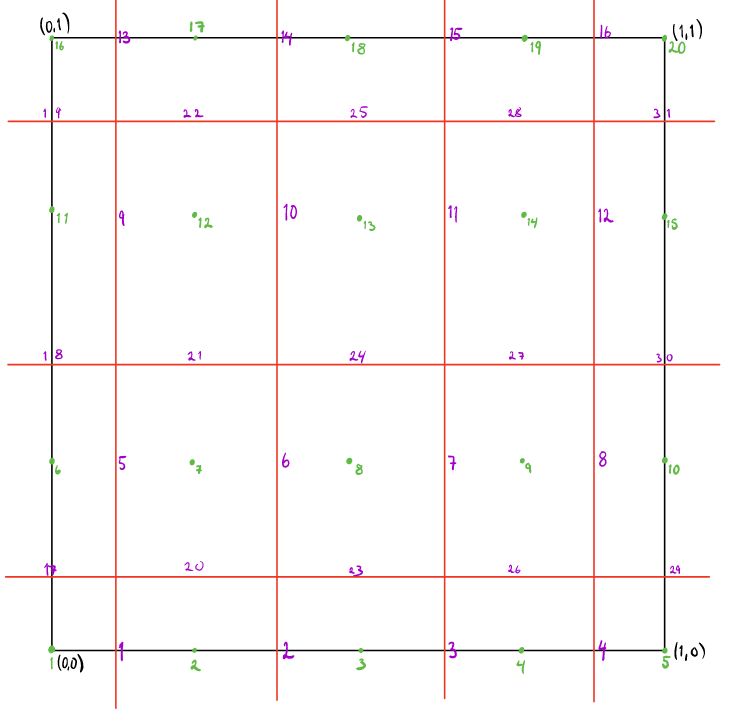
\includegraphics[scale=0.24]{grid.png}
            \end{figure}
        \end{columns}
    \end{frame}

    \begin{frame}{The numerical method: the divergence}
        Recall that
        \begin{equation*}
            \Delta \cdot \bm{q} = f
        \end{equation*}
        By Green's Theorem, in each cell $w$
        \begin{equation*}
            \oint_{\delta w} \bm{q} \cdot \hat{\bm{n}} ds = \iint_w \Delta \cdot \bm{q} dA = \iint_w f dA
        \end{equation*}
        Dividing by $\Delta x \Delta y$, we can approximate the double integral by $f$.
        \begin{equation*}
            \frac{1}{\Delta x \Delta y} (r_7 \Delta y + r_{24} \Delta x - r_6 \Delta y - r_{23}\Delta x) = v_8
        \end{equation*}
        \begin{figure}
            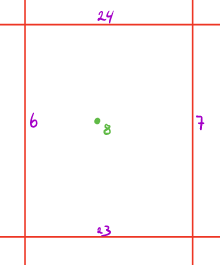
\includegraphics[scale=0.24]{cell.png}
        \end{figure}
    \end{frame}

    \begin{frame}{The numerical method: the system}
        We just have to solve for $v$
        \begin{equation*}
            D \cdot \underbrace{(-K \odot G) 
            \begin{bmatrix}
                v_1 \\
                v_2 \\
                v_3 \\
                \vdots \\
            \end{bmatrix}}_{\bm{r}}
            = 
            \begin{bmatrix}
                f_1 \\
                f_2 \\
                f_3 \\
                \vdots
            \end{bmatrix}
        \end{equation*}
    \end{frame}
\end{document}